% Choose one to switch between slides and handout
\documentclass[]{beamer}
%\documentclass[handout]{beamer}

% Video Meta Data
\title{Bitcoin, Blockchain and Cryptoassets}
\subtitle{Transaction Overview}
\author{Prof. Dr. Fabian Schär}
\institute{University of Basel}

% Config File
% Packages
\usepackage[utf8]{inputenc}
\usepackage{hyperref}
\usepackage{gitinfo2}
\usepackage{tikz}
\usepackage{amsmath}
\usepackage{bibentry}
\usepackage{xcolor}
\usepackage{colortbl} % Add colour to LaTeX tables
\usepackage{caption}
\usepackage[export]{adjustbox}
\usepackage{pgfplots} \pgfplotsset{compat = 1.17}

% Color Options
\definecolor{highlight}{rgb}{0.65,0.84,0.82}
\definecolor{focus}{rgb}{0.72, 0, 0}

% Beamer Template Options
\beamertemplatenavigationsymbolsempty
\setbeamertemplate{footline}[frame number]
\setbeamercolor{structure}{fg=black}
\setbeamercolor{footline}{fg=black}
\setbeamercolor{title}{fg=black}
\setbeamercolor{frametitle}{fg=black}
\setbeamercolor{item}{fg=black}
\setbeamercolor{}{fg=black}
\setbeamercolor{bibliography item}{fg=black}
\setbeamercolor*{bibliography entry title}{fg=black}
\setbeamertemplate{items}[square]
\setbeamertemplate{enumerate items}[default]
\captionsetup[figure]{labelfont={color=black},font={color=black}}
\captionsetup[table]{labelfont={color=black},font={color=black}}

\setbeamertemplate{bibliography item}{\insertbiblabel}

% Link Icon Command
\newcommand{\link}{%
    \tikz[x=1.2ex, y=1.2ex, baseline=-0.05ex]{%
        \begin{scope}[x=1ex, y=1ex]
            \clip (-0.1,-0.1)
                --++ (-0, 1.2)
                --++ (0.6, 0)
                --++ (0, -0.6)
                --++ (0.6, 0)
                --++ (0, -1);
            \path[draw,
                line width = 0.5,
                rounded corners=0.5]
                (0,0) rectangle (1,1);
        \end{scope}
        \path[draw, line width = 0.5] (0.5, 0.5)
            -- (1, 1);
        \path[draw, line width = 0.5] (0.6, 1)
            -- (1, 1) -- (1, 0.6);
        }
    }

% Read Git Data from Github Actions Workflow
% Defaults to gitinfo2 for local builds
\IfFileExists{gitInfo.txt}
	{\input{gitInfo.txt}}
	{
		\newcommand{\gitRelease}{(Local Release)}
		\newcommand{\gitSHA}{\gitHash}
		\newcommand{\gitDate}{\gitAuthorIsoDate}
	}

% Custom Titlepage
\defbeamertemplate*{title page}{customized}[1][]
{
  \vspace{-0cm}\hfill
\includegraphics[width=2.5cm]{../config/logo_cif}
  
\includegraphics[width=1.9cm]{../config/seal_wwz}
  \\ \vspace{2em}
  \usebeamerfont{title}\textbf{\inserttitle}\par
  \usebeamerfont{title}\usebeamercolor[fg]{title}\insertsubtitle\par  \vspace{1.5em}
  \small\usebeamerfont{author}\insertauthor\par
  \usebeamerfont{author}\insertinstitute\par \vspace{2em}
  \usebeamercolor[fg]{titlegraphic}\inserttitlegraphic
    \tiny \noindent \texttt{Release Ver.: \gitRelease}\\ 
    \texttt{Version Hash: \gitSHA}\\
    \texttt{Version Date: \gitDate}\\ \vspace{1em}
  \link \href{https://github.com/cifunibas/Bitcoin-Blockchain-Cryptoassets/blob/main/slides/intro.pdf}
  {Get most recent version}\\
  \link \href{https://github.com/cifunibas/Bitcoin-Blockchain-Cryptoassets/blob/main/slides/intro.pdf}
  {Watch video lecture}\\ \vspace{1em}
  License: \texttt{Creative Commons Attribution-NonCommercial-ShareAlike 4.0 International}\\\vspace{2em}
  
\includegraphics[width = 1.2cm]{../config/license}
}

% tikzlibraries
\usetikzlibrary{decorations.pathreplacing}
\usetikzlibrary{decorations.markings}
\usetikzlibrary{positioning}

%caption font
\captionsetup{font=footnotesize}

%%%%%%%%%%%%%%%%%%%%%%%%%%%%%%%%%%%%%%%%%%%%%%
%%%%%%%%%%%%%%%%%%%%%%%%%%%%%%%%%%%%%%%%%%%%%%
\begin{document}


%%
\thispagestyle{empty}
\begin{frame}[noframenumbering]
	\titlepage
\end{frame}
%%%


%%%
\begin{frame}{Structure of a Transaction}
	\centering
	\begin{figure}
	 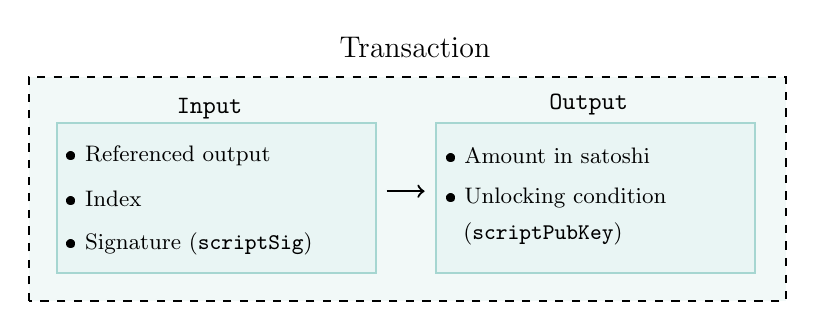
\begin{tikzpicture}[scale=0.9, every node/.style={scale=0.9}]
    
        \filldraw[yshift=-0.05cm, xshift=0.1cm,color = highlight!15, thick, draw=black, dashed] (-4,-4) rectangle ++(304pt,90pt) ;
    
        \filldraw[yshift=-0.05cm, xshift=0.1cm,color = highlight!25, thick, draw=highlight] (-3.6,-3.6) rectangle ++(128pt,60pt) ;
    
    \draw[->,thick] (1.15,-2.5) -- (1.685,-2.5) ;
    
    \draw[color=black] plot (-1.35,-1.6)   node[above] {\texttt{Input}};
    \draw[color=black] plot (-3.5,-2)   node[right] {\small{\textbullet{} {Referenced output}}};
    \draw[color=black] plot (-3.5,-2.6)   node[right] {\small{\textbullet{} Index}};
    \draw[color=black] plot (-3.5,-3.25)   node[right] {\small{\textbullet{} Signature (\texttt{scriptSig})}};
    \draw[color=black] plot (1.55,-0.2) node [below]
    {\large{{Transaction}}};
    
    
        \filldraw[yshift=-0.05cm, xshift=0.1cm,color = highlight!25, thick, draw=highlight] (1.75,-3.6) rectangle ++(128pt,60pt) ;
    
    \draw[color=black] plot (4,-1.55)   node[above] {\texttt{Output}};
    \draw[color=black] plot (1.85,-2)   node[right] {\small{\textbullet{} Amount in satoshi}};
    \draw[color=black] plot (1.85,-2.6)   node[right] {\small{\textbullet{} Unlocking condition}};
    \draw[color=black] plot (2,-3.1)   node[right] {\small{ (\texttt{scriptPubKey})}};
    %\draw[color=black] plot (1.95,-3.2)   node[right] {\small{\textbullet{} Signatur / Lösung}};
    
    \end{tikzpicture}

	\end{figure} 
\vspace{1em}
\begin{itemize}
  	\item<2->{Transaction must contain at least one in- and output.}
  	\item<3->{Sum of inputs must be at least as high as sum of outputs.}
\end{itemize}
\end{frame}	
%%%


%%%
\begin{frame}{UTXO model}

\begin{columns}
  \begin{column}{0.7\textwidth}
    \begin{figure}[h!]
    \center
     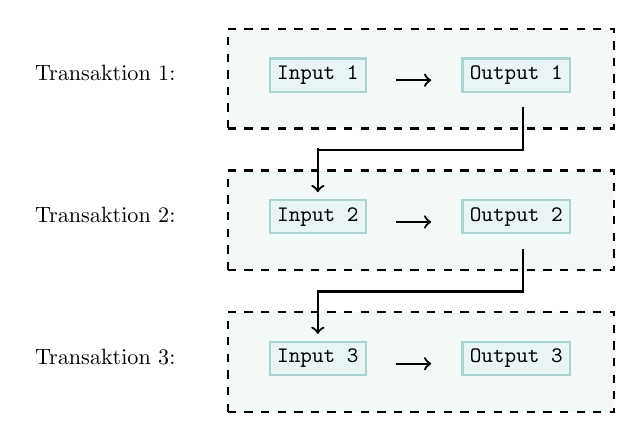
\begin{tikzpicture}[domain=-8:8,scale=0.9, every node/.style={scale=0.8}]
      
      
      \draw[color=black] plot (-3,3)   node[below, rotate = 0] {Transaktion 1:};
      \draw[color=black] plot (-3,1)   node[below, rotate = 0] {Transaktion 2:};
      \draw[color=black] plot (-3,-1)   node[below, rotate = 0] {Transaktion 3:};
      
        \filldraw[yshift=-0.05cm, xshift=0.1cm,color = highlight!15, thick, draw=black, dashed] (-1.37,2.05) rectangle ++(155pt,40pt) ;
      
      \draw[color=black] plot (0,3)   node[fill=highlight!25, thick, draw=highlight,below, rotate = 0] {\texttt{Input 1}};
      \draw[->,thick] (1.1,2.68) -- (1.6,2.68) ;
      \draw[color=black] plot (2.8,3) node [fill=highlight!25, thick, draw=highlight,below, rotate = 0]
      {\texttt{Output 1}};
      
      
        \filldraw[yshift=-0.05cm, xshift=0.1cm,color = highlight!15, thick, draw=black, dashed] (-1.37,0.05) rectangle ++(155pt,40pt) ;
      
      \draw[color=black] plot (0,1)   node[fill=highlight!25, thick, draw=highlight,below, rotate = 0] {\texttt{Input 2}};
      \draw[->,thick] (1.1,0.68) -- (1.6,0.68) ;
      \draw[color=black] plot (2.8,1) node [fill=highlight!25, thick, draw=highlight,below, rotate = 0]
      {\texttt{Output 2}};
      
      \draw[thick] (2.9,2.3) -- (2.9,1.7);
      \draw[thick] (2.915,1.7) -- (0,1.7);
      \draw[->,thick] (0,1.7175) -- (0,1.1);
      
      
        \filldraw[yshift=-0.05cm, xshift=0.1cm,color = highlight!15, thick, draw=black, dashed] (-1.37,-1.95) rectangle ++(155pt,40pt) ;
      
      \draw[color=black] plot (0,-1)   node[fill=highlight!25, thick, draw=highlight,below, rotate = 0] {\texttt{Input 3}};
      \draw[->,thick] (1.1,-1.32) -- (1.6,-1.32) ;
      \draw[color=black] plot (2.8,-1) node [fill=highlight!25, thick, draw=highlight,below, rotate = 0]
      {\texttt{Output 3}};
      
      \draw[thick] (2.9,0.3) -- (2.9,-0.3);
      \draw[thick] (2.915,-0.3) -- (0,-0.3);
      \draw[->,thick] (0,-0.2825) -- (0,-0.9);
      
\end{tikzpicture}

    \end{figure}
  \end{column}
  
  \begin{column}{0.3\textwidth}
  Only Output 3 is a \texttt{UTXO}.
  \end{column}
\end{columns}
\end{frame}
%\begin{itemize}
    %\item{Output can only be referenced once as input}
    %\item{Unspent transaction output = UTXO}
    %\item{UTXO's are the system's value storage}
    %\item{Stored on the blockchain and RAM of every full-node}
%\end{itemize} 
%\end{frame}       
%%%


%%%
\begin{frame}{Transaction Types}
\begin{columns}

\column{0.5\textwidth}
	\vspace{1cm}
	\begin{figure}
		%forwarding transaction

%%
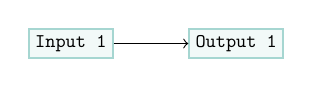
\begin{tikzpicture}[domain=-3:3,scale=0.7, every node/.style={scale=0.7}]
     
      \draw[color=black] plot (0,2)   node[fill=highlight!15, thick, draw=highlight,below, rotate = 0] (Input) {\texttt{Input 1}};
                   
      \draw[color=black] plot (3,2)   node[fill=highlight!15, thick, draw=highlight,below, rotate = 0] (Output) {\texttt{Output 1}};
 
 \draw[ -> ] (Input) -- (Output);       
\end{tikzpicture}
%%
		\vspace{2.5em}
		\caption*{forwarding}
	\end{figure} 
	\vspace{0.4cm}
	\begin{figure}
		% dividing transaction type

%%
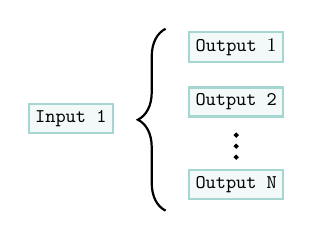
\begin{tikzpicture}[domain=-3:3,scale=0.7, every node/.style={scale=0.7}]
 
      \draw[color=black] plot (0.5,1.7)   node[fill=highlight!15, thick, draw=highlight,below, rotate = 0] {\texttt{Input 1}};
     
      
\draw[color=black] plot (3.5,3)   node[fill=highlight!15, thick, draw=highlight,below, rotate = 0] {\texttt{Output $1$}};
      \draw[color=black] plot (3.5,2)   node[fill=highlight!15, thick, draw=highlight,below, rotate = 0] {\texttt{Output 2}};
        \filldraw[color=black] (3.5,1.12) circle (1pt) ;
        \filldraw[color=black] (3.5,0.92) circle (1pt) ;
        \filldraw[color=black] (3.5,0.72) circle (1pt) ;
      \draw[color=black] plot (3.5,0.5)   node[fill=highlight!15, thick, draw=highlight,below, rotate = 0] {\texttt{Output N}};
      
      \draw [decorate,decoration={mirror, brace,amplitude=10pt},xshift=-8pt,yshift=0pt,thick]
      (2.5,3.05) -- (2.5,-0.25); %node [thick,black,midway,xshift=-1.6cm,fill=scheme!15,draw=scheme] 
      %{\texttt{Input 1}};
\end{tikzpicture}
%%
		\caption*{splitting}
	\end{figure}
\column{0.5\textwidth}
	\begin{figure}
		% aggregating transaction type

%%
\begin{figure}[b!]
\centering
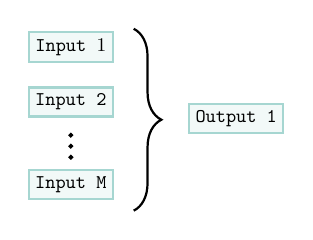
\begin{tikzpicture}[domain=-3:3,scale=0.7, every node/.style={scale=0.7}]
      %Aggregierende trx
      \draw[color=black] plot (0,3)   node[fill=highlight!15, thick, draw=highlight,below, rotate = 0] {\texttt{Input $1$}};
      \draw[color=black] plot (0,2)   node[fill=highlight!15, thick, draw=highlight,below, rotate = 0] {\texttt{Input 2}};
        \filldraw[color=black] (0,1.12) circle (1pt) ;
        \filldraw[color=black] (0,0.92) circle (1pt) ;
        \filldraw[color=black] (0,0.72) circle (1pt) ;
      \draw[color=black] plot (0,0.5)   node[fill=highlight!15, thick, draw=highlight,below, rotate = 0] {\texttt{Input M}};
      
\draw [decorate,decoration={brace,amplitude=10pt},xshift=4pt,yshift=0pt,thick]
      (1,3.05) -- (1,-0.25); %node [thick,black,midway,xshift=1.7cm,fill=scheme!15,draw=scheme] 
      %{\texttt{Output 1}};
          
      \draw[color=black] plot (3,1.7)   node[fill=highlight!15, thick, draw=highlight,below, rotate = 0] {\texttt{Output 1}};      
\end{tikzpicture} \\
aggregating
\end{figure}
%%
		\caption*{aggregating}
	\end{figure}
	\vspace{0.5cm}
	\begin{figure}
		%% m to n transaction type

%%
\begin{figure}[b!]
\centering
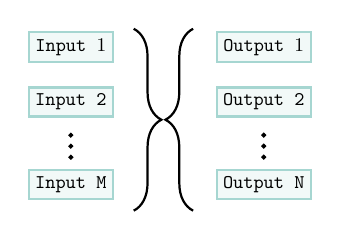
\begin{tikzpicture}[domain=-3:3,scale=0.7, every node/.style={scale=0.7}]
      
      \draw[color=black] plot (0,3)   node[fill=highlight!15, thick, draw=highlight,below, rotate = 0] {\texttt{Input $1$}};
      \draw[color=black] plot (0,2)   node[fill=highlight!15, thick, draw=highlight,below, rotate = 0] {\texttt{Input 2}};
        \filldraw[color=black] (0,1.12) circle (1pt) ;
        \filldraw[color=black] (0,0.92) circle (1pt) ;
        \filldraw[color=black] (0,0.72) circle (1pt) ;
      \draw[color=black] plot (0,0.5)   node[fill=highlight!15, thick, draw=highlight,below, rotate = 0] {\texttt{Input M}};
      
      \draw [decorate,decoration={brace,amplitude=10pt},xshift=4pt,yshift=0pt,thick]
      (1,3.05) -- (1,-0.25); 
      
\draw[color=black] plot (3.5,3)   node[fill=highlight!15, thick, draw=highlight,below, rotate = 0] {\texttt{Output $1$}};
      \draw[color=black] plot (3.5,2)   node[fill=highlight!15, thick, draw=highlight,below, rotate = 0] {\texttt{Output 2}};
        \filldraw[color=black] (3.5,1.12) circle (1pt) ;
        \filldraw[color=black] (3.5,0.92) circle (1pt) ;
        \filldraw[color=black] (3.5,0.72) circle (1pt) ;
      \draw[color=black] plot (3.5,0.5)   node[fill=highlight!15, thick, draw=highlight,below, rotate = 0] {\texttt{Output N}};
      
      \draw [decorate,decoration={mirror, brace,amplitude=10pt},xshift=-8pt,yshift=0pt,thick]
      (2.5,3.05) -- (2.5,-0.25); 
\end{tikzpicture} \\
m to n
\end{figure}
%%
		\caption*{combined (m to n)}
	\end{figure}
	
\end{columns}
\end{frame}
%%%

%%%
\begin{frame}{Example: Transaction Hierarchy}
\resizebox{\textwidth}{!}{

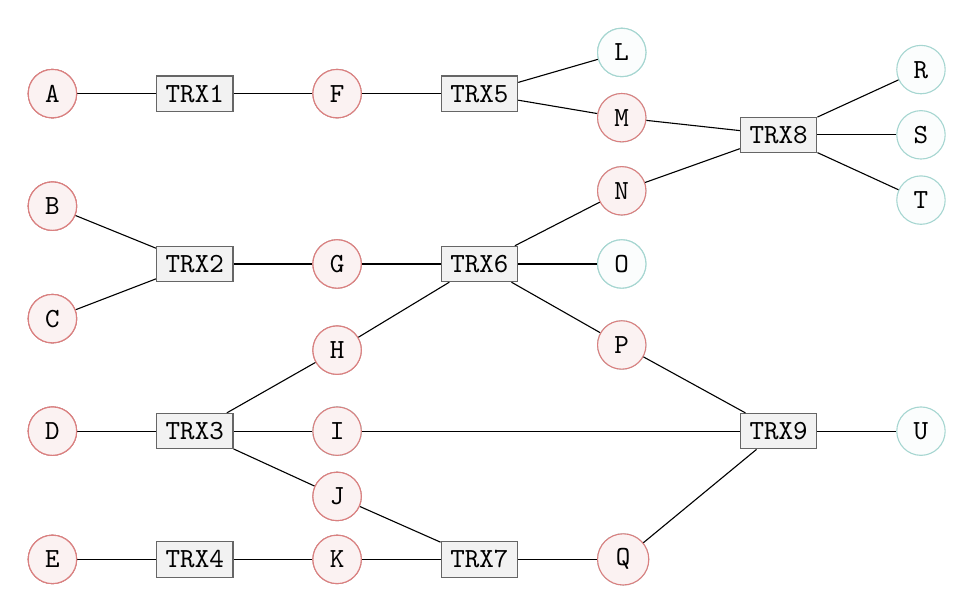
\begin{tikzpicture}[
      roundnode1/.style = {circle,  draw=highlight, fill=highlight!5},
      roundnode2/.style = {circle,  draw=focus!50, fill=focus!5},
      squarednode/.style = {rectangle, draw=black!60, fill=black!5},
      ]

     % 1st slide
    \uncover<1->{
    \node[roundnode1]    (nodeA)                                  {\texttt{A}};
    \node[roundnode1]    (nodeB)        [below=8mm of nodeA]      {\texttt{B}};
    \node[roundnode1]    (nodeC)        [below=8mm of nodeB]      {\texttt{C}};
    \node[roundnode1]    (nodeD)        [below=8mm of nodeC]      {\texttt{D}};
    \node[roundnode1]    (nodeE)        [below=10mm of nodeD]     {\texttt{E}};
    }
   
    % 2nd slide
    \uncover<2->{
    \node[roundnode2]    (nodeA)                                    {\texttt{A}};
    \node[roundnode2]    (nodeB)        [below=8mm of nodeA]        {\texttt{B}};
    \node[roundnode2]    (nodeC)        [below=8mm of nodeB]        {\texttt{C}};
    \node[roundnode2]    (nodeD)        [below=8mm of nodeC]        {\texttt{D}};
    \node[roundnode2]    (nodeE)        [below=10mm of nodeD]       {\texttt{E}};
    
    \node[squarednode]  (TRX1)          [right =of nodeA]           {\texttt{TRX1}}; 
    \node[squarednode]  (TRX2)          [below =17mm of TRX1]       {\texttt{TRX2}};
    \node[squarednode]  (TRX3)          [right =of nodeD]           {\texttt{TRX3}};
    \node[squarednode]  (TRX4)          [right =of nodeE]           {\texttt{TRX4}};
    
    \node[roundnode1]    (nodeF)        [right =of TRX1]            {\texttt{F}};
    \node[roundnode1]    (nodeG)        [right =of TRX2]            {\texttt{G}};
    \node[roundnode1]    (nodeI)        [right =of TRX3]            {\texttt{I}};
    \node[roundnode1]    (nodeH)        [above =4mm of nodeI]       {\texttt{H}};
    \node[roundnode1]    (nodeJ)        [below =2mm of nodeI]       {\texttt{J}};
    \node[roundnode1]    (nodeK)        [right =of TRX4]            {\texttt{K}};
    
    \draw[-] (nodeA) -- (TRX1);
    \draw[-] (nodeB) -- (TRX2);
    \draw[-] (nodeC) -- (TRX2);
    \draw[-] (nodeD) -- (TRX3);
    \draw[-] (nodeE) -- (TRX4);
    
    \draw[-] (TRX1) -- (nodeF);
    \draw[-] (TRX2) -- (nodeG);
    \draw[-] (TRX3) -- (nodeH);
    \draw[-] (TRX3) -- (nodeI);
    \draw[-] (TRX3) -- (nodeJ);
    \draw[-] (TRX4) -- (nodeK);
    }
   
    % 3rd slide
    \uncover<3->{
    \node[roundnode2]    (nodeA)                                  {\texttt{A}};
    \node[roundnode2]    (nodeB)        [below=8mm of nodeA]      {\texttt{B}};
    \node[roundnode2]    (nodeC)        [below=8mm of nodeB]      {\texttt{C}};
    \node[roundnode2]    (nodeD)        [below=8mm of nodeC]      {\texttt{D}};
    \node[roundnode2]    (nodeE)        [below=10mm of nodeD]     {\texttt{E}};
    
    \node[squarednode]  (TRX1)          [right =of nodeA]           {\texttt{TRX1}}; 
    \node[squarednode]  (TRX2)          [below =17mm of TRX1]       {\texttt{TRX2}};
    \node[squarednode]  (TRX3)          [right =of nodeD]           {\texttt{TRX3}};
    \node[squarednode]  (TRX4)          [right =of nodeE]           {\texttt{TRX4}};
    
    \node[roundnode2]    (nodeF)        [right =of TRX1]           {\texttt{F}};
    \node[roundnode2]    (nodeG)        [right =of TRX2]           {\texttt{G}};
    \node[roundnode1]    (nodeI)        [right =of TRX3]           {\texttt{I}};
    \node[roundnode2]    (nodeH)        [above =4mm of nodeI]      {\texttt{H}};
    \node[roundnode2]    (nodeJ)        [below =2mm of nodeI]      {\texttt{J}};
    \node[roundnode2]    (nodeK)        [right =of TRX4]           {\texttt{K}};
    
    \node[squarednode]  (TRX5)          [right =of nodeF]          {\texttt{TRX5}}; 
    \node[squarednode]  (TRX6)          [right =of nodeG]          {\texttt{TRX6}};
    \node[squarednode]  (TRX7)          [right =of nodeK]          {\texttt{TRX7}};
    
    \node[roundnode1]    (nodeO)        [right =of TRX6]           {\texttt{O}};
    \node[roundnode1]    (nodeN)        [above =3mm of nodeO]      {\texttt{N}};
    \node[roundnode1]    (nodeM)        [above =3mm of nodeN]      {\texttt{M}};
    \node[roundnode1]    (nodeL)        [above =2mm of nodeM]      {\texttt{L}};
    \node[roundnode1]    (nodeP)        [below =4mm of nodeO]      {\texttt{P}};
    \node[roundnode1]    (nodeQ)        [right =of TRX7]           {\texttt{Q}};
    
    \draw[-] (nodeF) -- (TRX5);
    \draw[-] (nodeG) -- (TRX6);
    \draw[-] (nodeH) -- (TRX6);
    \draw[-] (nodeJ) -- (TRX7);
    \draw[-] (nodeK) -- (TRX7);
    
    \draw[-] (TRX5) -- (nodeL);
    \draw[-] (TRX5) -- (nodeM);
    \draw[-] (TRX6) -- (nodeN);
    \draw[-] (TRX6) -- (nodeO);
    \draw[-] (TRX6) -- (nodeP);
    \draw[-] (TRX7) -- (nodeQ);
    }
    
    %4th slide
    \uncover<4->{
    \node[roundnode2]    (nodeA)                                    {\texttt{A}};
    \node[roundnode2]    (nodeB)        [below=8mm of nodeA]        {\texttt{B}};
    \node[roundnode2]    (nodeC)        [below=8mm of nodeB]        {\texttt{C}};
    \node[roundnode2]    (nodeD)        [below=8mm of nodeC]        {\texttt{D}};
    \node[roundnode2]    (nodeE)        [below=10mm of nodeD]       {\texttt{E}};
    
    \node[squarednode]  (TRX1)          [right =of nodeA]           {\texttt{TRX1}}; 
    \node[squarednode]  (TRX2)          [below =17mm of TRX1]       {\texttt{TRX2}};
    \node[squarednode]  (TRX3)          [right =of nodeD]           {\texttt{TRX3}};
    \node[squarednode]  (TRX4)          [right =of nodeE]           {\texttt{TRX4}};
    
    \node[roundnode2]    (nodeF)        [right =of TRX1]            {\texttt{F}};
    \node[roundnode2]    (nodeG)        [right =of TRX2]            {\texttt{G}};
    \node[roundnode2]    (nodeI)        [right =of TRX3]            {\texttt{I}};
    \node[roundnode2]    (nodeH)        [above =4mm of nodeI]       {\texttt{H}};
    \node[roundnode2]    (nodeJ)        [below =2mm of nodeI]       {\texttt{J}};
    \node[roundnode2]    (nodeK)        [right =of TRX4]            {\texttt{K}};
    
    \node[squarednode]  (TRX5)          [right =of nodeF]          {\texttt{TRX5}}; 
    \node[squarednode]  (TRX6)          [right =of nodeG]          {\texttt{TRX6}};
    \node[squarednode]  (TRX7)          [right =of nodeK]          {\texttt{TRX7}};
    
    \node[roundnode1]    (nodeO)        [right =of TRX6]            {\texttt{O}};
    \node[roundnode2]    (nodeN)        [above =3mm of nodeO]       {\texttt{N}};
    \node[roundnode2]    (nodeM)        [above =3mm of nodeN]       {\texttt{M}};
    \node[roundnode1]    (nodeL)        [above =2mm of nodeM]       {\texttt{L}};
    \node[roundnode2]    (nodeP)        [below =4mm of nodeO]       {\texttt{P}};
    \node[roundnode2]    (nodeQ)        [right =of TRX7]            {\texttt{Q}};
    
    \node[squarednode]  (TRX9)          [right = 48mm of nodeI]    {\texttt{TRX9}};
    \node[squarednode]  (TRX8)          [above = 33mm of TRX9]     {\texttt{TRX8}};
    
    \node[roundnode1]    (nodeS)        [right =of TRX8]            {\texttt{S}};
    \node[roundnode1]    (nodeR)        [above =2mm of nodeS]       {\texttt{R}};
    \node[roundnode1]    (nodeT)        [below =2mm of nodeS]       {\texttt{T}};
    \node[roundnode1]    (nodeU)        [right =of TRX9]            {\texttt{U}};
    
    \draw[-] (nodeM) -- (TRX8);
    \draw[-] (nodeN) -- (TRX8);
    \draw[-] (nodeP) -- (TRX9);
    \draw[-] (nodeQ) -- (TRX9);
    \draw[-] (nodeI) -- (TRX9);
    
    \draw[-] (TRX8) -- (nodeR);
    \draw[-] (TRX8) -- (nodeS);
    \draw[-] (TRX8) -- (nodeT);
    \draw[-] (TRX9) -- (nodeU);
    } 
 
\end{tikzpicture}

}
\end{frame}
%%%


%%%
\begin{frame}{Input $\neq$ Output ?}
If the input value does not correspond to the output value, there are the following two possibilities:
\vspace{1em}
\begin{itemize}
    \item<1->{Output Value $>$ Input Value $\rightarrow$ Transaction invalid}
    \item<2->{Output Value $<$ Input Value $\rightarrow$ Miner gets difference}
    \end{itemize} 
    \vspace{1.5em}
\uncover<3->{A higher fee usually results in faster confirmation / block inclusion.}
\end{frame}
%%%


\end{document}
